\documentclass[aspectratio=169,10pt,dvipsnames]{beamer} 
\usepackage{graphicx}
\usepackage{tabularx}
\usepackage{array}
\usepackage[most]{tcolorbox}
\usepackage{mathtools}
\usepackage{stackengine}
\usepackage{algorithmic}
\usepackage{epstopdf}
\usepackage{lipsum}
\usepackage{pifont}
\usepackage{algorithm}
\usepackage{tikz}
\usepackage{animate}
\usetikzlibrary{decorations.pathreplacing}
\usepackage[export]{adjustbox}
\renewcommand{\thealgorithm}{}
\usetikzlibrary{matrix}
\usepackage{natbib} 
\usepackage{bibentry}
\newcommand{\amin}{\mathop{\text{argmin}}}
\newcommand{\forestgreen}{\color{forestgreen}}
\newcommand{\red}{\color{red}}
\newcommand{\blue}{\color{blue}}
\newcommand{\bx}{\boldsymbol{x}}
\newcommand{\blambda}{\boldsymbol{\lambda}}
\newcommand{\by}{\boldsymbol{y}}
\newcommand{\bz}{\boldsymbol{z}}
\newcommand{\bX}{\boldsymbol{X}}
\newcommand{\bY}{\boldsymbol{Y}}
\newcommand{\bZ}{\boldsymbol{Z}}
\newcommand{\bv}{\boldsymbol{v}}
\newcommand{\bu}{\boldsymbol{u}}
\newcommand{\bxi}{\boldsymbol{\xi}}
\newcommand{\bpsi}{\boldsymbol{\psi}}
\newcommand{\bzeta}{\boldsymbol{\zeta}}
\newcommand{\boldsymbolu}{\boldsymbol{\mu}}
\newcommand{\bQ}{\boldsymbol{Q}}
\newcommand{\bS}{\boldsymbol{S}}
\newcommand{\bT}{\boldsymbol{T}}
\newcommand{\bF}{\boldsymbol{F}}
\newcommand{\bG}{\boldsymbol{G}}
\newcommand{\bd}{\boldsymbol{d}}
\newcommand{\bp}{\boldsymbol{p}}
\newcommand{\bff}{\boldsymbol{f}}
\newcommand{\bc}{\boldsymbol{c}}
\newcommand{\bg}{\boldsymbol{g}}
\newcommand{\bA}{\boldsymbol{A}}
\newcommand{\bB}{\boldsymbol{B}}
\newcommand{\bSigma}{\boldsymbol{\Sigma}}
\newcommand{\bC}{\boldsymbol{C}}
\newcommand{\bE}{\boldsymbol{E}}
\newcommand{\bh}{{\boldsymbol{h}}}
\newcommand{\bH}{{\boldsymbol{H}}}
\newcommand{\bJ}{{\boldsymbol{J}}}
\newcommand{\bR}{{\boldsymbol{R}}}
\newcommand{\bn}{\boldsymbol{n}}
\newcommand{\br}{\boldsymbol{r}}
\newcommand{\bl}{\boldsymbol{l}}
\newcommand{\bI}{\boldsymbol{I}}
\newcommand{\bzero}{\boldsymbol{0}}
\newcommand{\st}{\mathop{\text{s.t.}}}
\newcommand{\diag}{\mathop{\text{\normalfont diag}}}
\newcommand{\aminmax}{\mathop{\text{\normalfont argminmax}}}
\newcommand{\interior}{\mathop{\text{\normalfont interior}}}
\newcommand{\ReH}{\mathop{\text{\normalfont Re}}}

\setbeamertemplate{navigation symbols}{}

\newcommand\blfootnotefirst[1]{%
  \begingroup
  \renewcommand\thefootnote{}\footnote{\color{darkgray}\tiny\vspace{-.13in}\hspace{-.32in}#1}%
  \addtocounter{footnote}{-1}%
  \endgroup
}

\newcommand\blfootnote[1]{%
  \begingroup
  \renewcommand\thefootnote{}\footnote{\color{darkgray}\tiny\vspace{-.02in}\hspace{-.32in}#1}%
  \addtocounter{footnote}{-1}%
  \endgroup
}

\newcommand\with[1]{%
  \begingroup
  \renewcommand\thefootnote{}\footnote{\hspace{-.32in}\normalfont Joint Work with #1}%
  \addtocounter{footnote}{-1}%
  \endgroup
}
\renewcommand\footnoterule{}

%% Colors
\definecolor{forestgreen}{rgb}{0.13, 0.55, 0.13}
\definecolor{green2}{rgb}{0, 0.8, 0}
\definecolor{UWGray}{RGB}{90,90,90}
\definecolor{UWRed}{RGB}{38,72,161}
\setbeamerfont{author}{series=\bfseries}
\setbeamerfont{title}{series=\bfseries}
\setbeamerfont{frametitle}{series=\bfseries}
\setbeamerfont{block title}{size={}}
\setbeamercolor{block title}{fg=UWRed}
\newcommand{\green}{\color{green2}}
\newcommand{\UWgray}{\color{UWGray}}
\newcommand{\UWred}{\color{UWRed}}
\usepackage{cmbright}
% \usefonttheme{professionalfonts} % using non standard fonts for beamer
% \usepackage[utf8]{inputenc} 
% \usepackage[T1]{fontenc}
% \usepackage[frenchb]{babel}
% \usepackage{setspace}
\usepackage{color}
\usepackage{listings}
\lstdefinelanguage{Julia}%
{morekeywords={abstract,break,case,catch,const,continue,do,else,elseif,%
end,export,false,for,function,immutable,import,importall,if,in,%
macro,module,otherwise,quote,return,switch,true,try,type,typealias,%
using,while,@threads,@optinode,@variable,@constraint,@NLnodeconstraint,@linkconstraint,@objective,@optiedge},%
sensitive=true,%
alsoother={$},%$
morecomment=[l]\#,%
morecomment=[n]{\#=}{=\#},%
morestring=[s]{"}{"},%
morestring=[m]{'}{'},%
}[keywords,comments,strings]%
\definecolor{codegreen}{rgb}{0,0.6,0}
\definecolor{codegray}{rgb}{0.5,0.5,0.5}
\definecolor{codepurple}{rgb}{0.58,0,0.82}
\definecolor{backcolour}{rgb}{0.95,0.95,0.92}
\lstdefinestyle{mystyle}{
backgroundcolor=\color{backcolour},   
commentstyle=\color{codegreen},
keywordstyle=\color{magenta},
numberstyle=\tiny\color{codegray},
stringstyle=\color{codepurple},
basicstyle=\ttfamily\footnotesize,
breakatwhitespace=false,         
breaklines=true,                 
captionpos=b,                    
keepspaces=true,                 
numbers=left,                    
numbersep=5pt,                  
showspaces=false,                
showstringspaces=false,
showtabs=false,                  
tabsize=2
}
\lstset{%
language         = Julia,
basicstyle       = \ttfamily,
keywordstyle     = \bfseries\color{blue},
stringstyle      = \color{magenta},
commentstyle     = \color{ForestGreen},
showstringspaces = false,
style            = mystyle
}

\usepackage{pgfplots}
\usepackage{tikz}
\usetikzlibrary{calc}
\usetikzlibrary{colorbrewer}
\pgfplotsset{colormap/blackwhite}

\tikzset{%
  add/.style args={#1 and #2}{to path={%
 ($(\tikztostart)!-#1!(\tikztotarget)$)--($(\tikztotarget)!-#2!(\tikztostart)$)%
  \tikztonodes}}
} 

\beamersetrightmargin{0.025\paperwidth}
\beamersetleftmargin{0.025\paperwidth}

\usepackage{animate}


\definecolor{emph}{rgb}{0.2,0.2,0.7}
\setbeamertemplate{footline}[frame number]
\setbeamertemplate{subsection in toc}{\hspace*{2em}{\footnotesize \inserttocsectionnumber.\inserttocsubsectionnumber.~\inserttocsubsection\par}}
\setbeamertemplate{section in toc}{\inserttocsectionnumber.~\inserttocsection\par}
\usepackage{hyperref}

\usepackage{times}
\usepackage{DejaVuSansMono}

\usepackage{enumitem}
\setitemize{label=\usebeamerfont*{itemize item}%
  \usebeamercolor[fg]{itemize item}
  \usebeamertemplate{itemize item}}

\newcommand{\backupbegin}{
   \newcounter{finalframe}
   \setcounter{finalframe}{\value{framenumber}}
}
\newcommand{\backupend}{
   \setcounter{framenumber}{\value{finalframe}}
}
\usetikzlibrary{positioning, fadings, backgrounds}

\usepackage{multirow}
\newcommand{\reference}[1]{%
  \tikz[remember picture,overlay,align=center]{s
    \node[anchor=south west,color=darkgray,font=\tiny,align=left,inner sep=1] at (current page.south west) {#1};
  }%
}
\usepackage{wrapfig}
\title{ExaModels and MadNLP: Open-Source Software Infrastructure for Accelerated Nonlinear Optimization on GPUs}
\author{Sungho Shin$^\dag$, François Pacaud$^\ddag$, and Mihai Anitescu$^\dag$} 
\date{\small
  $^\dag$Mathematics and Computer Science Division, Argonne National Laboratory\\
  $^\ddag$Centre Automatique et Systèmes, Mines Paris - PSL, Paris, France
}
\begin{document}
\maketitle

We are delighted to submit our nominations for the COIN-OR Cup,
highlighting our contributions of {\bf ExaModels} \cite{examodels} and
{\bf MadNLP} \cite{madnlp} in the field of computational
infrastructure for operations research, specifically in the area of
nonlinear programming (NLP). Our open-source software packages
represent a significant breakthrough in efficiently solving
large-scale NLPs by leveraging the capabilities of modern GPU
hardware.  In this document, we address the primary challenges and
opportunities for optimization software development in 2023,
particularly within the context of accelerated computing. We elucidate
how ExaModels and MadNLP collectively address technical obstacles and
capitalize on the advantages offered by modern accelerated
computing. Furthermore, we emphasize the remarkable performance
enhancements achieved in solving real-world nonlinear optimization
problems at scale. A noteworthy example of such progress is our recent
accomplishment in accelerating alternating current (AC) optimal power
flow (OPF) problems by up to ten times compared to state-of-the-art
tools. Finally, we discuss how our development lays the foundation for
the advancement in various topics in operations research and unlocks
new possibilities.

\paragraph{Challenges and Opportunities} In recent years, the
scalability of deep learning has experienced significant advancements,
primarily due to the utilization of NVIDIA
GPUs, which have demonstrated remarkable success in constructing
large-scale AI models. Additionally, in the public domain, GPU
accelerators have provided a substantial portion of the computational
power for next-generation leadership HPC systems such as Frontier and
Aurora, achieving the milestone of one exaflop per second.  While GPUs
have proven highly effective in various scientific computing areas
like machine learning and high-fidelity simulations, integrating them
into constrained NLP algorithms has encountered
considerable challenges. Specifically, the seamless translation of
sparse automatic differentiation (AD) and sparse linear solver
routines to GPU architecture has been recognized to be particularly
challenging.  This is because conventional sparse AD and matrix
factorization algorithms are designed for CPUs and heavily rely on
serial computation, making them unsuitable for the single-instruction,
multiple-data (SIMD) parallelism employed by GPU architectures (see
Figure \ref{fig:simd}, left).

While GPU computation can accelerate several parts of the optimization
process straightforwardly, the slow data transfer between host and
device memory hinders the ad-hoc implementation of GPU accelerations
(Figure \ref{fig:simd}, right). To fully exploit the potential offered
by modern GPU hardware, it is crucial to develop a comprehensive
computational framework for optimization on GPUs. This requires
keeping the problem data and the solver's intermediate computational
data reside exclusively within device memory, with the majority of
operations executed on the GPU. Consequently, the development of a
comprehensive NLP solution framework that performs
all necessary computations, including AD, optimization, and linear
algebra, exclusively on GPUs becomes imperative.  To address these
challenges, ExaModels and MadNLP offer a comprehensive solution
framework for NLP. They enable AD and NLP solution
exclusively on GPUs, while linear algebra computation is performed by
the external library (e.g., cuSOLVER), allowing for the full
utilization of GPUs.

\begin{figure}[t]
  \centering 
  \scalebox{.82}{
    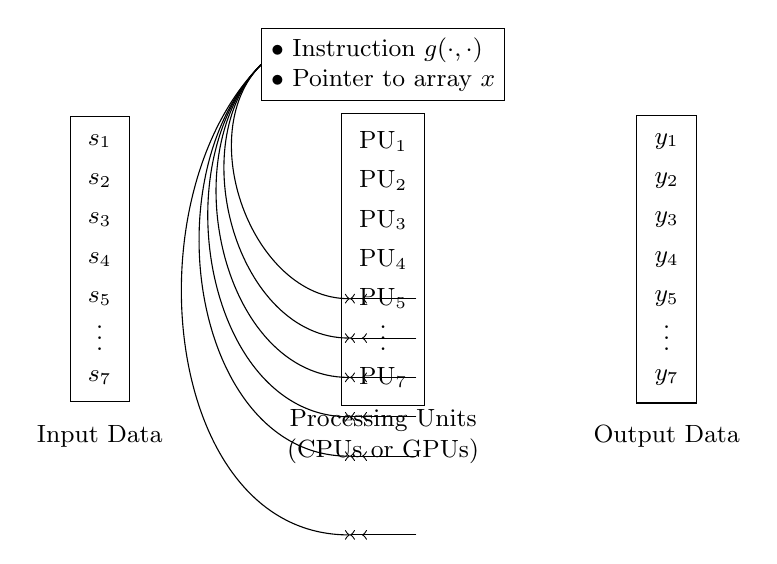
\begin{tikzpicture}[remember picture, scale=.9, font=\small]
    \node[draw,align=left] (I) at (0,2.75) {
      $\bullet$ Instruction $g(\cdot,\cdot)$\\
      $\bullet$ Pointer to array $x$
    };
    \node[draw] at (-4,0) {
      \tikz{
        \foreach\x in {1,2,3,4,5,7}{
          \node (A\x) at (0,-\x/2) {$s_{\x}$};
        }
        \node at (0,-2.9) {$\vdots$};
      }
    };
    \node[draw] at (0,0) {
      \tikz{
        \foreach\x in {1,2,3,4,5,7}{
          \node (B\x) at (0,-\x/2) {$\text{PU}_{\x}$};
        }
        \node at (0,-2.9) {$\vdots$};
      }
    };
    \node[draw] at (4,0) {
      \tikz{
        \foreach\x in {1,2,3,4,5,7}{
          \node (C\x) at (0,-\x/2) {$y_{\x}$};
        }
        \node at (0,-2.9) {$\vdots$};
      }
    };
    \foreach\x in {1,2,3,4,5,7}{
      \draw[->] (A\x.east) -- (B\x.west);
      \draw[->] (B\x.east) -- (C\x.west);
      \draw[->] (I.west) to [out=-135,in=180] (B\x.west);
    }
    \node at (-4,-2.5) {Input Data};
    \node[align=center] at (0,-2.5) {Processing Units\\(CPUs or GPUs)};
    \node at (4,-2.5) {Output Data};
  \end{tikzpicture} 
  }
  \scalebox{.87}{
  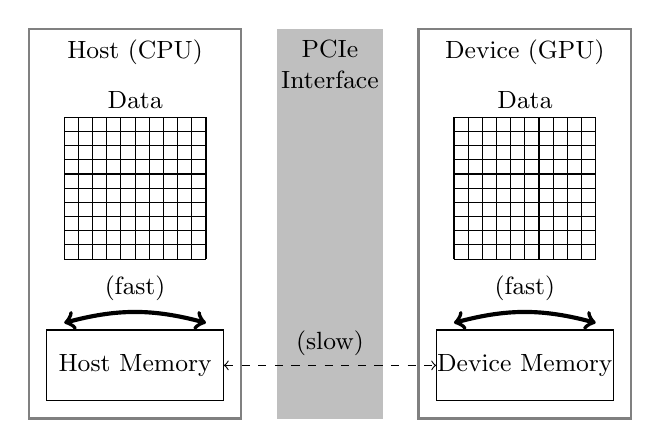
\begin{tikzpicture}[remember picture, scale=.9, font=\small]

    \fill[lightgray] (3.25,-.75) rectangle (4.75,4.75) node[black,midway,align=center,yshift=57.5] {PCIe\\Interface};
    \draw[gray,thick] (-.25,-.75) rectangle (2.75,4.75) node[black,midway,align=center,yshift=62] {Host (CPU)};
    \draw[gray,thick] (5.25,-.75) rectangle (8.25,4.75) node[black,midway,align=center,yshift=62] {Device (GPU)};

    \node[align=center] at (1.25, 3.75) {Data};
    \node[align=center] at (6.75, 3.75) {Data};

    % Host Memory
    \draw (0,-.5) rectangle (2.5,.5) node[midway] {Host Memory};

    % Device Memory
    \draw (5.5,-.5) rectangle (8,.5) node[midway] {Device Memory};


    % Arrow with Dashed Line
    \draw[<->, dashed] (2.5, 0) -- (5.5, 0) node[midway, above, align=center] {(slow)};
    \draw[<->, line width=1.5] (.25, .6) to [in=165, out =15] node[midway, above, align=center] {(fast)}(2.25, .6) ;
    \draw[<->, line width=1.5] (5.75, .6) to [in=165, out =15] node[midway, above, align=center] {(fast)}(7.75, .6) ;

    \def\rows{10}
    \def\cols{10}
    \def\elementwidth{2}
    \foreach \xshift/\yshift in {.25/1.5, 5.75/1.5} {
      % Draw Grid
      \foreach \i in {0,...,\rows} {
        \draw (\xshift, \yshift+\i*\elementwidth/\rows) -- (\xshift+\elementwidth, \yshift+\i*\elementwidth/\rows);
      }
      \foreach \i in {0,...,\cols} {
        \draw (\xshift+\i*\elementwidth/\cols, \yshift) -- (\xshift+\i*\elementwidth/\cols, \yshift+\elementwidth);
      }
    }
  \end{tikzpicture}
  }
  \caption{Schematics of host and device memory architectures (left) and SIMD parallelism (right).}
  \label{fig:simd}
\end{figure}


\paragraph{ExaModels}

ExaModels is an algebraic modeling and AD system embedded in the Julia
Language, specialized for the SIMD abstraction of nonlinear
programs. This system is designed based on the repetitive structure
commonly found in large-scale NLPs. For example, AC OPF problems,
which may have millions of variables and constraints, can be expressed
using just 15 computational patterns. By enforcing the creation of
models through specifying repetitive patterns, ExaModels preserves the
parallelizable structure within model equations and facilitates
parallel automatic differentiation. Writing models in ExaModels
automatically enables GPU compatibility, which is especially
beneficial as optimization models are often implemented by domain
experts who may not fully understand the internals of algebraic
modeling systems and NLP solvers.  This makes ExaModels a powerful
modeling platform for scalable computations.


By enabling efficient computation of derivatives on GPUs, ExaModels
provides exceptional performance, surpassing existing tools like AMPL
(AD backend of Pyomo) and JuMP by more than two orders of
magnitude. Our numerical results demonstrate that conventional
algebraic modeling systems struggle to efficiently compute derivatives
of model equations (Table \ref{tab:num}), and they are incompatible
with GPU operations (Table \ref{tbl:portability}). In contrast,
ExaModels provides a convenient framework for users to inform the AD
backend about the parallelizable structure, and in turn, efficient,
parallelized AD can be performed in the backend.


\paragraph{MadNLP}

MadNLP is a versatile NLP solver capable of
handling various problem data structures. By leveraging the modularity
provided by the key features of the Julia Language, such as multiple
dispatch and just-in-time compilation, MadNLP offers great flexibility
in handling different types of data structures while retaining the
sophistication of the algorithm. Importantly, with this approach, we can avoid
re-implementing interior point solver every time for each data types,
which in turn ensures that the operations performed are mathematically
equivalent to those in the mature, extensively tested existing code
base. MadNLP has started as a port of Ipopt (an open-source nonlinear
optimziation solver running on CPUs) in the Julia Language, but over
the past four years, it has expanded beyond its initial scope and now
offers a range of capabilities not supported by state-of-the-art NLP
solvers. These include solving dense optimization problems, handling
different numerical precisions, working with different forms of KKT
systems, managing diverse array data types (including GPU device
arrays), and utilizing various Hessian approximation strategies, such
as different variants of BFGS methods.

Recently, we have discovered that the condensed-space interior point
method (IPM) with an inequality relaxation strategy is particularly
effective for solving large-scale NLPs, like AC optimal power flow, up
to moderate precisions. This strategy efficiently addresses the
challenges posed by sparse matrix factorization on GPUs, as the
condensed KKT systems can be factorized without numerical pivoting,
which has previously hindered GPU utilization in the large-scale
optimization regime.  Furthermore, MadNLP offers diverse approaches
for handling KKT systems with special structures, via reduction
strategies \cite{pacaud2023accelerating} and Schur complement decomposition
strategies \cite{pacaud2023parallel}.



\paragraph{Performance Highlights}

Our numerical results, summarized in Table \ref{tab:num} (for detailed
results, please refer to \cite{shin2023accelerating}), clearly
demonstrate the significant potential of using GPUs. Specifically,
when applied to AC OPF problems, which are one of the most important
applications of NLP, we have achieved significant performance
enhancements. The GPU-based solutions achieve speedups of over 10
times compared to CPU-based state-of-the-art tools. Notably, ExaModels
enables derivative evaluations that are up to two orders of magnitude
faster, and the use of the condensed-space IPM strategy in MadNLP
greatly improves linear algebra computation speed. Furthermore, we
have also explored the utilization of these methods in reduced-space
OPF \cite{pacaud2023accelerating} and model predictive control (MPC)
\cite{cole2023exploiting}, where we have achieved similar degrees of
speedup.

 
\begin{table}[t]
  \begin{center}
    \begin{tabular}{|l|c|c|ccc|ccc|}
  \hline
  \multirow{3}{*}{\textbf{Case}}
  & \multirow{3}{*}{\# vars}
  & \multirow{3}{*}{\# cons}
  & \multicolumn{3}{c|}{\textbf{MadNLP+ExaModels+cuSOLVER}}
  & \multicolumn{3}{c|}{\textbf{Ipopt+AMPL+Ma27}}
  \\
  & & &\multicolumn{3}{c|}{\textbf{(GPU$^*$)}} &\multicolumn{3}{c|}{\textbf{(CPU$^{**}$)}}
  \\
  \cline{4-9}
  & & 
  & \quad \# iter \quad& \quad AD$^\dag$  \quad&  \quad total$^\dag$ \quad
    & \quad \# iter \quad& \quad AD$^\dag$  \quad&  \quad total$^\dag$ \quad
  \\
  \hline
  10480\_goc 
  &  96.8k
  & 150.9k
  & 70 
  &  0.13
  & 14.26
    & 64 
      & 16.93
                                               & 38.04
  \\

  13659\_pegase 
  & 117.4k
  & 170.6k
  & 63 
  &  0.12
  &  7.15
    & 64 
      & 19.70
                                               & 35.66
  \\

  19402\_goc 
  & 179.6k
  & 281.7k
  & 79 
  &  0.17
  & 23.28
    & 70 
      & 36.50
                                               & 95.34
  \\

  24464\_goc 
  & 203.4k
  & 313.6k
  & 63 
  &  0.11
  & 70.63
    & 58 
      & 33.50
                                               & 70.15
  \\

  30000\_goc 
  & 208.6k
  & 307.8k
  & 162 
  &  0.33
  & 22.05
    & 180 
      & 101.98
                                               & 249.81
  \\
    \hline  
\end{tabular}
    \vspace{-1em}
    \footnotesize
    $^\dag$Wall time (sec) measured by Julia. $^\ddag$CPU time (sec) reported by Ipopt.  
  \end{center}
  \caption{Numerical Performance of ExaModels and MadNLP for solving AC OPF problems}
  \label{tab:num}
\end{table}

\paragraph{Portability}


While NVIDIA currently leads in terms of computing power and mature
implementation of low-level operations, especially with CUDA
libraries, we aim to provide support for alternative architectures as
well. This is crucial because many next-generation exascale
high-performance computing architectures will be based on AMD and
Intel accelerator devices. Furthermore, by supporting diverse
platforms, we hope to drive the attention of chip makers towards the
operations research field and encourage better support for software
infrastructure in implementing operations research software.

Table \ref{tbl:portability} provides an overview of the current state
of portability for our tools and other existing open-source software
tools. ExaModels.jl already supports all major architectures, while
MadNLP.jl currently only supports NVIDIA GPUs. However, we have a
clear roadmap to extend support to all major accelerator
architectures, including NVIDIA, AMD, and Intel GPUs. The portability
is enabled by KernelAbstractions.jl, a Julia package that facilitates
the portable implementation of GPU kernels. 

\begin{table}[t]
  \begin{center}
    \scalebox{0.72}{
      \begin{tabular}{|c|c|cccccc|}
        \hline
        &&CPU (single) &CPU (multi)& NVIDIA & AMD & Intel& Apple\\
        \hline
        \multirow{3}{*}{Algebraic Modeling Platforms}& {\bf AMPL}& \cmark& \xmark& \xmark& \xmark& \xmark& \xmark\\
        &{\bf JuMP}& \cmark& \xmark& \xmark& \xmark& \xmark& \xmark\\
        &{\bf ExaModels}& \cmark& \cmark& \cmark& \cmark& \cmark& \xmark\\ 
        \hline
        \multirow{2}{*}{NLP Solvers} & {\bf Ipopt}& \cmark& \xmark& \xmark& \xmark& \xmark& \xmark\\
        & {\bf MadNLP} & \cmark& \xmark& \cmark& \xmark& \xmark& \xmark\\
        \hline
      \end{tabular}
    }
  \end{center}
  \caption{The current status on the portability of the NLP frameworks.}
  \label{tbl:portability}
\end{table}

\paragraph{Expected Impacts in Applications}

\begin{itemize}
\item \textit{Energy Infrastructures}: Enhancing the scalability of
optimization methods is crucial for improving the resilience of energy
system operations. We have demonstrated the ability of MadNLP with
multiple GPUs to solve large-scale security-constrained AC OPF
problems effectively \cite{pacaud2023parallel}. This showcases the
potential of ExaModels and MadNLP to enhance the scalability of NLP by
utilizing GPU capabilities.

\item \textit{Model Predictive Control}: MPC has been widely used for
optimization-based control in various settings, such as chemical
processes, energy systems, and robotics. However, the effectiveness of
MPC is often limited by the efficiency of optimization solvers,
especially when short sampling times are required. Our results have
shown that MadNLP running on GPUs can solve such problems with high
efficiency \cite{cole2023exploiting}. Moving forward, we plan to
implement the extension packages for control problems so that control
community can take advantage of accelerated NLP frameworks.

\item \textit{Machine Learning Surrogate Models}: An exciting future
direction is the integration of neural network surrogate models into
constrained optimization algorithms (a proof-of-concept presented in
\cite{shin2023constrained}). GPU acceleration plays a crucial role in
these applications, considering the complexity of real-world AI
models. MadNLP offers the necessary capabilities through the native
handling of device arrays as well as dense KKT systems with various
quasi-Newton strategies. We intend to explore these problems further
and provide extensions for surrogate modeling with GPU acceleration.

\end{itemize}

\paragraph{Closing Remarks} ExaModels and MadNLP provide computational
infrastructures for operations research that align with the era of
accelerated computing, which we believe the COIN-OR cup aims to
recognize. By addressing critical challenges and introducing new
strategies, these packages significantly extend the boundaries of
computational infrastructure for operations research. We are confident
that these contributions will resonate within the operations research
community and beyond, opening up new possibilities in applications
such as energy systems, control, and machine learning. With great
enthusiasm, we nominate ExaModels and MadNLP for the COIN-OR cup, in
recognition of their impact on the field.

\bibliographystyle{plain} 
\bibliography{main}
\end{document}